\documentclass[11pt]{beamer}

\usepackage[utf8]{inputenc} % Encodage des sources
\usepackage[frenchb]{babel} % Typographie francaise
\usepackage[T1]{fontenc} % Pour la police
\usepackage{lmodern} % Pour la police
\usepackage{graphicx} % Affichage d'images
\usepackage{color} % Couleur
\usepackage{multicol} % Plusieurs colonnes
\usepackage{hyperref} % Liens
\hypersetup{
	colorlinks,
	citecolor=blue,
	filecolor=black,
	linkcolor=white,
	urlcolor=blue
}

\usepackage{listings} % Codes
\lstset{
frame=single,
frameround=tttt,
keywordstyle=\bfseries \ttfamily \color{blue},
commentstyle=\color[rgb]{0.133,0.545,0.133},
stringstyle=\ttfamily \color{red},
showstringspaces=true,
tabsize=4,
basicstyle=\footnotesize \ttfamily,
numberstyle=\footnotesize \ttfamily,
numbers=left,
breaklines=true,
breakatwhitespace=true,
aboveskip={\baselineskip},
belowskip={\baselineskip},
columns=fixed,
extendedchars=true,
}

\usetheme{Warsaw}
\setbeamertemplate{navigation symbols}{}
\addtobeamertemplate{footline}{\hspace{0.45em} \insertframenumber \hspace{0.45em}}

\title{Vers une carte d'identité des langages de programmation}
\author{Sylvain {\sc Joubert} \hspace{1cm} Philippe {\sc Mignot}}
\date{22 Mars 2011} 

\begin{document} %%%%%%%%%%%%%%%%%%%%%%%%%%%%%%%%%%%%%%%%%%%%%%%%%%%%%%%

\frame{ %---------------------------------------------------------------
\begin{center}
PVETE 2010
\end{center}

\maketitle


\includegraphics[scale=0.4]{img/cc}\\
\tiny Œuvre mise à disposition selon les termes de la \href{http://creativecommons.org/licenses/by-nc-sa/3.0/}{Licence Creative Commons BY-NC-SA 3.0} \normalsize
}

\frame{\frametitle{Sujet} %------------------------------------------
\begin{figure}
	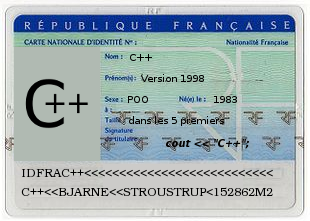
\includegraphics[scale=0.4]{img/carte}
\end{figure}

\begin{itemize}[<+->]
\item Problématique
	\begin{itemize}[<+->]
	\item Identifier et définir les traits caractéristiques d'un langage de programmation
	\item Structurer ces données afin d'en extraire une carte d'identité représentant la notion de langage
	\end{itemize}
\item Contexte
	\begin{itemize}[<+->]
	\item Différents types de langages informatiques
	\item Restriction aux langages de programmation
	\end{itemize}
\end{itemize}
}

\frame{\frametitle{Carte d'identité} %-------------------------------
\begin{multicols}{2}
\begin{itemize}
\item<1-> Généralités
	\begin{itemize}
	\item Nom
	\item Version
	\item Date de création
	\item Créateur(s)
	\item Logo
	\vspace*{1em}
	\end{itemize}
\item<2-> Paradigmes
	\begin{itemize}
	\item impératif
	\item orienté objet
	\item …
	\vspace*{1em}
	\end{itemize}
\item<3-> Typage
	\begin{itemize}
	\item Fort | faible
	\item Statique | dynamique
	\item Explicite | implicite
	\end{itemize}
\columnbreak

\item<4-> Divers
	\begin{itemize}
	\item Turing-complétude
	\item Évaluation
	\item Gestion de la mémoire
	\vspace*{\fill}
	\end{itemize}
\item<5-> Communauté
	\begin{itemize}
	\item Popularité
	\item Implémentations
	\vspace*{\fill}
	\end{itemize}
\item<6-> Code
	\begin{itemize}
	\item Code objet
	\item Hello world!
	\vspace*{\fill}
	\end{itemize}
\end{itemize}
\end{multicols}
}

\frame[containsverbatim]{\frametitle{Exemple : Perl} %-------------------------------
\begin{multicols}{2}
\begin{figure}
	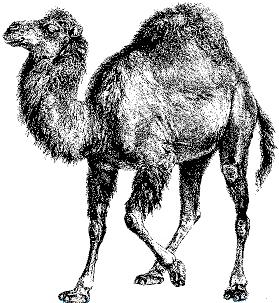
\includegraphics[scale=0.2]{img/perl.jpg}
\end{figure}
\begin{itemize}
\footnotesize
\item Généralités
	\begin{itemize}
	\scriptsize
	\item Nom : Perl
	\item Version : 5.12.3
	\item Date de création : 1987
	\item Créateur : Larry {\sc Wall}
	\end{itemize}
\item Paradigmes
	\begin{itemize}
	\scriptsize
	\item impératif
	\item orienté objet
	\item fonctionnel
	\item …
	\end{itemize}
\item Typage
	\begin{itemize}
	\scriptsize
	\item faible
	\item dynamique
	\item partiellement explicite
	\end{itemize}
\columnbreak

\item Divers
	\begin{itemize}
	\scriptsize
	\item Turing-complétude : oui
	\item Évaluation : stricte
	\item Gestion de la mémoire : par l'implémentation
	\end{itemize}
\item Communauté
	\begin{itemize}
	\scriptsize
	\item Popularité : populaire (10 premières places)
	\item Implémentations : Perl, Strawberry Perl, ActivePerl
	\end{itemize}
\item Code
	\begin{itemize}
	\scriptsize
	\item Code objet : code source (interprété)
	\item Hello world! :
	\end{itemize}
\begin{lstlisting}[language=perl]
# Hello world! en Perl
print "Hello world!";
\end{lstlisting}
\end{itemize}
\end{multicols}
\normalsize
}

\frame{\frametitle{Exemple : Piet} %-------------------------------
\begin{multicols}{2}
\begin{itemize}
\item Généralités
	\begin{itemize}
	\item Nom : Piet
	\item Date de création : avant 1990
	\item Créateur : David {\sc Morgan-Mar}
	\end{itemize}
\item Paradigmes
	\begin{itemize}
	\item à pile
	\end{itemize}
\item Typage
	\begin{itemize}
	\item fort
	\item statique
	\item implicite
	\end{itemize}
\item Divers
	\begin{itemize}
	\item Turing-complétude : oui
	\item Évaluation : stricte
	\item Gestion de la mémoire : par l'implémentation
	\end{itemize}
\columnbreak

\item Communauté
	\begin{itemize}
	\item Popularité : exotique
	\end{itemize}
\item Code
	\begin{itemize}
	\item Code objet : code source (interprété)
	\item Hello world! :
	\end{itemize}
\vspace*{\fill}
\begin{center}
\includegraphics<2->[scale=0.5]{img/piet}
\end{center}
\vspace*{\fill}
\end{itemize}
\end{multicols}
}

\frame{\frametitle{Conclusion} %--------------------------------
\begin{alertblock}{- -}<2->
\begin{itemize}
\item Difficultés à trouver et spécifier les valeurs des caractéristiques pour certains langages
\item Subjectivité dans le choix des entrées de la carte d'identité
\end{itemize}
\end{alertblock}

\begin{exampleblock}{++}<3->
\begin{itemize}
\item Possibilité de concevoir une base de données
\item Choix d'un langage facilité
\item Extension à d'autres types de langages ?
\end{itemize}
\end{exampleblock}
}

\frame[containsverbatim]{ %---------------------------------------------------------------
\begin{lstlisting}
++++++++++[>+>+++>+++++++>++++++++++<<<<-]>>>
+++++++++++.>+++++++++++++++++.----------------.
++++++++++++++.+.-----------.++++++.-.+++++.<<++.>
------------------.
\end{lstlisting}

\begin{center}
\begin{LARGE}
Questions ?
\end{LARGE}
\end{center}
}

\end{document}
